\documentclass[12pt]{article}
\input{/Users/circle/Documents/博一下/homework/setting.tex}
\setcounter{secnumdepth}{2}
\usepackage{autobreak}
\usepackage{amsmath}
\setlength{\parindent}{2em}
\graphicspath{{../}}
\ziju{0.1pt}

%pdf文件设置
\hypersetup{
	pdfauthor={袁磊祺},
	pdftitle={计算流体力学作业12}
}

\title{
		\vspace{-1in} 	
		\usefont{OT1}{bch}{b}{n}
		\normalfont \normalsize \textsc{\LARGE Peking University}\\[0.2cm] % Name of your university/college \\ [25pt]
		\horrule{0.5pt} \\[0.2cm]
		\huge \bfseries{计算流体力学作业12} \\[-0.2cm]
		\horrule{2pt} \\[0.2cm]
}
\author{
		\normalfont 								\normalsize
		College of Engineering \quad 2001111690  \quad 袁磊祺\\	\normalsize
        \today
}
\date{}

\begin{document}

% %%%%%%%%%%%%%%%%%%%%%%%%%%%%%%%%%%%%%%%%%%%%%%
\captionsetup[figure]{name={图},labelsep=period}
\captionsetup[table]{name={表},labelsep=period}
\renewcommand\contentsname{目录}
\renewcommand\listfigurename{插图目录}
\renewcommand\listtablename{表格目录}
\renewcommand\refname{参考文献}
\renewcommand\indexname{索引}
\renewcommand\figurename{图}
\renewcommand\tablename{表}
\renewcommand\abstractname{摘\quad 要}
\renewcommand\partname{部分}
\renewcommand\appendixname{附录}
\def\equationautorefname{式}%
\def\footnoteautorefname{脚注}%
\def\itemautorefname{项}%
\def\figureautorefname{图}%
\def\tableautorefname{表}%
\def\partautorefname{篇}%
\def\appendixautorefname{附录}%
\def\chapterautorefname{章}%
\def\sectionautorefname{节}%
\def\subsectionautorefname{小小节}%
\def\subsubsectionautorefname{subsubsection}%
\def\paragraphautorefname{段落}%
\def\subparagraphautorefname{子段落}%
\def\FancyVerbLineautorefname{行}%
\def\theoremautorefname{定理}%
\crefname{figure}{图}{图}
\crefname{equation}{式}{式}
\crefname{table}{表}{表}
%%%%%%%%%%%%%%%%%%%%%%%%%%%%%%%%%%%%%%%%%%%

\maketitle

\section{A}


考虑二维的守恒律方程
\begin{equation}
	u_{t}+f(u)_{x}+g(u)_{y}=0, \quad u(x, y, 0)=u_{0}(x, y)
	\label{eq:11}
\end{equation}
给定空间网格剖分: $x_{j}=j h_{x}, y_{k}=k h_{y}$, 其中网格步长 $h_{x}$ 可不等于 $h_{y} .$试导出/写出WENO有限差分方法和WENO有限体积方法(时间方向采用显式Euler). [提 示 : 基 于 解$ u$ 插值/重构,或者基于通量 $f, g$ 的插值/重构; 要求:在截断误差意义下至少具有空间三阶精度.]


Here we define
\begin{equation}
	h_x = \Delta x_i, \quad h_y = \Delta y_i,\quad I_{ij} = [x_{i-\frac{1}{2}},x_{i+\frac{1}{2}}]\times [y_{j-\frac{1}{2}},y_{j+\frac{1}{2}}].
\end{equation}


\subsection{Reconstruction from cell averages.\cite{Shu1998}}

The approximation problem we will face, in solving hyperbolic conservation laws using cell averages (finite volume schemes), is still the following reconstruction problem.

Two dimensional reconstruction. Given the cell averages of a function $v(x, y)$
\begin{equation}
	\quad \bar{v}_{i j} \equiv \frac{1}{\Delta x_{i} \Delta y_{j}} \int_{y_{j-\frac{1}{2}}}^{y_{j+\frac{1}{2}}} \int_{x_{i-\frac{1}{2}}}^{x_{i+\frac{1}{2}}} v(\xi, \eta) d \xi d \eta, \quad i=1,2, \ldots, N_{x}, j=1,2, \ldots, N_{y}
\end{equation}
find a polynomial $p_{i j}(x, y)$, preferably of degree at most $k-1$, for each cell $I_{i j}$, such that it is a $k$ -th order accurate approximation to the function $v(x, y)$ inside $I_{i j}$ :
\begin{equation}
	p_{i j}(x, y)=v(x, y)+O\left(\Delta^{k}\right), \quad(x, y) \in I_{i j}, i=1, \ldots, N_{x}, j=1, \ldots, N_{y}
\end{equation}
In particular, this gives approximations to the function $v(x, y)$ at the cell boundaries
\begin{equation}
	\begin{array}{l}
		v_{i+\frac{1}{2}, y}^{-}=p_{i j}\left(x_{i+\frac{1}{2}}, y\right), v_{i-\frac{1}{2}, y}^{+}=p_{i j}\left(x_{i-\frac{1}{2}}, y\right), i=1, \ldots, N_{x}, y_{j-\frac{1}{2}} \leq y \leq y_{j+\frac{1}{2}} \\
		v_{x, j+\frac{1}{2}}^{-}=p_{i j}\left(x, y_{j+\frac{1}{2}}\right), v_{x, j-\frac{1}{2}}^{+}=p_{i j}\left(x, y_{j-\frac{1}{2}}\right), j=1, \ldots, N_{y}, x_{i-\frac{1}{2}} \leq x \leq x_{i+\frac{1}{2}}
	\end{array}
\end{equation}
which are $k$ -th order accurate:
$\quad v_{i+\frac{1}{2}, y}^{\pm}=v\left(x_{i+\frac{1}{2}}, y\right)+O\left(\Delta^{k}\right), \quad i=0,1, \ldots, N_{x}, $ $ y_{j-\frac{1}{2}} \leq y \leq y_{j+\frac{1}{2}}$
and
\begin{equation}
	v_{x, j+\frac{1}{2}}^{\pm}=v\left(x, y_{j+\frac{1}{2}}\right)+O\left(\Delta^{k}\right), \quad j=0,1, \ldots, N_{y}, \quad x_{i-\frac{1}{2}} \leq x \leq x_{i+\frac{1}{2}}
\end{equation}


\subsection{Finite volume formulation in the scalar case.}

For finite volume schemes, or schemes based
on cell averages, we do not solve \cref{eq:11} directly, but its integrated version. We integrate \cref{eq:11} over the
interval $I_{i j}$ to obtain
\begin{equation}
	\begin{aligned}
		\frac{\dif \bar{u}_{i j}(t)}{\dif t}= & -\frac{1}{\Delta x_{i} \Delta y_{j}}\left(\int _ { y _ { j - \frac { 1 } { 2 } } } ^ { y _ { j + \frac { 1 } { 2 } } } f \left(u\left(x_{i+\frac{1}{2}}, y, t\right)\right) \dif y-\int_{y_{j-\frac{1}{2}}}^{y_{j+\frac{1}{2}}} f\left(u\left(x_{i-\frac{1}{2}}, y, t\right)\right) \dif y\right. \\
		                                      & \left.+\int_{x_{i-\frac{1}{2}}}^{x_{i+\frac{1}{2}}} g\left(u\left(x, y_{j+\frac{1}{2}}, t\right)\right) \dif x-\int_{x_{i-\frac{1}{2}}}^{x_{i+\frac{1}{2}}} g\left(u\left(x, y_{j-\frac{1}{2}}, t\right)\right) \dif x\right)
	\end{aligned}
	\label{eq:1pde}
\end{equation}
where
\begin{equation}
	\bar{u}_{i j}(t) \equiv \frac{1}{\Delta x_{i} \Delta y_{j}} \int_{y_{j-\frac{1}{2}}}^{y_{j+\frac{1}{2}}} \int_{x_{i-\frac{1}{2}}}^{x_{i+\frac{1}{2}}} u(\xi, \eta, t) \dif \xi \dif \eta
\end{equation}
is the cell average. Use explicit Euler time scheme
\begin{equation}
	\frac{\dif \bar{u}_{i j}(t)}{\dif t}=\frac{\bar{u}^{n+1}_{i j}(t)-\bar{u}^{n}_{i j}(t)}{\tau}
\end{equation}

We approximate \cref{eq:1pde} by the following conservative scheme
\begin{equation}
	\frac{\dif \bar{u}_{i j}(t)}{\dif t}=-\frac{1}{\Delta x_{i}}\left(\hat{f}_{i+\frac{1}{2}, j}-\hat{f}_{i-\frac{1}{2}, j}\right)-\frac{1}{\Delta y_{j}}\left(\hat{g}_{i, j+\frac{1}{2}}-\hat{g}_{i, j-\frac{1}{2}}\right)
	\label{eq:scheme}
\end{equation}where the numerical flux $\hat{f}_{i+\frac{1}{2}, j}$ is defined by
\begin{equation}
	\hat{f}_{i+\frac{1}{2}, j}=\sum_{\alpha} w_{\alpha} h\left(u_{i+\frac{1}{2}, y_{j}+\beta_{\alpha} \Delta y_{j}}^{-}, u_{i+\frac{1}{2}, y_{j}+\beta_{\alpha} \Delta y_{j}}^{+}\right)
	\label{eq:1fhat}
\end{equation}
where $\beta_{\alpha}$ and $w_{\alpha}$ are Gaussian quadrature nodes and weights, for approximating the integration in $y$ :
\begin{equation}
	\frac{1}{\Delta y_{j}} \int_{y_{j-\frac{1}{2}}}^{y_{j+\frac{1}{2}}} f\left(u\left(x_{i+\frac{1}{2}}, y, t\right)\right) \dif y
\end{equation}
inside the integral form of the PDE \cref{eq:1pde}, and $u_{i+\frac{1}{2}, y}^{\pm}$ are the $k$ -th order accurate reconstructed values obtained by ENO or WENO reconstruction, the superscripts $\pm$ imply the values are obtained within the cell $I_{i j}$ (for the superscript -) and the cell $I_{i+1, j}$ (for the superscript $+)$, respectively. The flux $\hat{g}_{i, j+\frac{1}{2}}$ is defined similarly by \cref{eq:1fhat}
\begin{equation}
	\hat{g}_{i, j+\frac{1}{2}}=\sum_{\alpha} w_{\alpha} h\left(u_{x_{i}+\beta_{\alpha} \Delta x_{i}, j+\frac{1}{2}}^{-} u_{x_{i}+\beta_{\alpha} \Delta x_{i}, j+\frac{1}{2}}^{+}\right)
	\label{eq:1ghat}
\end{equation}
for approximating the integration in $x$ :
\begin{equation}
	\frac{1}{\Delta x_{i}} \int_{x_{i-\frac{1}{2}}}^{x_{i+\frac{1}{2}}} g\left(u\left(x, y_{j+\frac{1}{2}}, t\right) d x\right.
\end{equation}
inside the integral form of the PDE \cref{eq:1pde}. $u_{x, j+\frac{1}{2}}^{\pm}$ are again the $k$ -th order accurate reconstructed values obtained by ENO or WENO reconstruction described before. $h$ is again the one dimensional monotone flux.

We summarize the procedure to build a finite volume ENO or WENO 2D scheme \cref{eq:scheme}, given the cell averages $\left\{\bar{u}_{i j}\right\}$ (we again drop the explicit reference to the time variable $t$ ), and a one dimensional monotone flux $h$, as follows:


\subsection{Procedure 3.1. Finite volume 2D scalar ENO and WENO.}


\begin{enumerate}
	\item Follow the procedures described in Sect. 3.2, to obtain ENO or WENO reconstructed values at the Gaussian points, $u_{i+\frac{1}{2}, y_{j}+\beta_{\alpha} \Delta y_{j}}^{\pm}$ and $u_{x_{i}+\beta_{\alpha} \Delta x_{i}, j+\frac{1}{2}}^{\pm}$ Notice that this step involves two one dimensional reconstructions, each one to remove a one dimensional cell average in one of the two directions. Also notice that the optimal weights used in the WENO reconstruction procedure are different for different Gaussian points indexed by $\alpha$;
	\item Compute the flux $\hat{f}_{i+\frac{1}{2}, j}$ and $\hat{g}_{i, j+\frac{1}{2}}$ using \cref{eq:1fhat,eq:1ghat};
	\item Form the scheme \cref{eq:scheme}.
\end{enumerate}




\section{B}

考虑对流扩散方程(Navier-Stokes方程对应的模型方程)
\begin{equation}
	u_{t}+a u_{x}=\nu u_{x x}, \quad u(x, 0)=u_{0}(x),
	\label{eq:21}
\end{equation}
其中 $a, \nu>0$ 是常数. 给定空间网格剖分: $x_{j}=j h, h$ 为网格步长.
\begin{enumerate}
	\item 讨论(空间导数采用二阶中心差商近似, 时间导数采用显式Euler)有限差分格式的稳定性[提示: Fourier方法或von Neumann方法]. 当 $0<\nu \ll 1$ 时, 该格式是否可以用于实际问题计算?
	\item 采用ENO/WENO离散,给出一个在截断误差意义下至少具有时空三阶精度的数值方法.
\end{enumerate}

\subsection{1}

采用如下方式进行离散
\begin{equation}
	u_t = \frac{u^{n+1}_{j}-u^{n}_{j}}{\tau},\quad u_x = \frac{u^n_{j+1}-u^n_{j-1}}{2h},\quad u_{xx} = \frac{u^n_{j+1}-2u^n_{j}+u^n_{j-1}}{h^2}
\end{equation}
\cref{eq:21}离散为
\begin{equation}
	\frac{u^{n+1}_{j}-u^{n}_{j}}{\tau} = -a\frac{u^n_{j+1}-u^n_{j-1}}{2h}+\nu \frac{u^n_{j+1}-2u^n_{j}+u^n_{j-1}}{h^2}
\end{equation}
\begin{equation}
	u^{n+1}_{j} = \tau \left( \frac{\nu}{h^2} - \frac{a}{2h} \right)u^n_{j+1} + \left( 1 - \frac{2\tau\nu}{h^2} \right)u^n_{j} + \tau \left( \frac{\nu}{h^2} + \frac{a}{2h} \right)u^n_{j-1}
	\label{eq:22}
\end{equation}
采用 Fourier 方法,将
\begin{equation}
	u^n_{j,k} = \xi^n_l \me^{\mi \beta jh}
\end{equation}
代入离散方程\cref{eq:22}得放大因子
\begin{equation}
	G(\beta,h) = 1+\frac{2\tau \nu}{h^2}\left( \cos \beta h-1 \right) - \frac{a\tau}{h} \sin(\beta h) \mi
\end{equation}
\begin{equation}
	\begin{aligned}
		\abs{G} = & \frac{-a^2 h^2 \tau^2 {\cos \left(\beta h\right)}^2 +a^2 h^2 \tau^2 +h^4 +4h^2 \nu\tau\cos \left(\beta h\right)-4h^2 \nu\tau+4\nu^2 \tau^2 {\cos \left(\beta h\right)}^2 }{h^4 } \\
		          & \frac{-8\nu^2 \tau^2 \cos \left(\beta h\right)+4\nu^2 \tau^2 }{}
	\end{aligned}
\end{equation}
当网格较密时,格式很可能是不稳定的。但是格式是可能稳定的,例如
\begin{equation}
	\frac{2\tau \nu}{h^2} = 1,\quad \frac{a\tau}{h} = 1
\end{equation}
时, $\abs{G}=1$.而当$0<\nu \ll 1$ 时,即高雷诺数情况,
\begin{equation}
	G(\beta,h) \approx 1 - \frac{a\tau}{h} \sin(\beta h) \mi
\end{equation}
此时$\abs{G}>1$所以是不稳定的。不可以用于实际计算。


\subsection{2 WENO3}

我们首先记一阶偏导对流项
\begin{equation}
	au_x = \left( au \right)_x = f_x,\quad f = au.
\end{equation}
二阶偏导扩散项
\begin{equation}
	\nu u_xx = (\nu u)_{xx} = b_{xx},\quad b(u) = \nu u.
\end{equation}

对于$f$,使用Steger-Warming 通量分裂方法是根据特征值 $\lambda_{i}$ 来完成的,首先将特征值分解为正负部分:
\begin{equation}
	\lambda_{i}^{+}=\frac{1}{2}\left(\lambda_{i}+\left|\lambda_{i}\right|\right), \quad \lambda_{i}^{-}=\frac{1}{2}\left(\lambda_{i}-\left|\lambda_{i}\right|\right) .
\end{equation}
进而将矩阵 $A$ 分为正负两部分
\begin{equation}
	A=T^{-1} \Lambda T=T^{-1}\left(\Lambda^{+}+\Lambda^{-}\right) T=A^{+}+A^{-},
\end{equation}
其中 $\Lambda, \Lambda^{\pm}$ 是对角线上是特征值的对角矩阵。于是正负通量为
\begin{equation}
	f^{+}=A^{+} U,
\end{equation}
例如 $r=2$ 时, 插值得到的可能 $f_{j+\frac{1}{2}}^{\pm}$ 为
\begin{equation}
	f_{j+\frac{1}{2}}^{+}=\left\{\begin{array}{l}
		-\frac{1}{2} f_{j-1}^{+}+\frac{3}{2} f_{j}^{+} \\
		\frac{1}{2} f_{j}^{+}+\frac{1}{2} f_{j+1}^{+},
	\end{array}, \quad f_{j+\frac{1}{2}}^{-}=\left\{\begin{array}{l}
		\frac{3}{2} f_{j+1}^{-}-\frac{1}{2} f_{j+2}^{-} \\
		\frac{1}{2} f_{j+1}^{-}+\frac{1}{2} f_{j}^{-}
	\end{array}\right.\right..
\end{equation}
相应的三阶WENO插值为
\begin{align}
	\hat{f}_{j+\frac{1}{2}}^{+} & =\omega_{1} \hat{f}_{j+\frac{1}{2}}^{(1),+}+\omega_{2} \hat{f}_{j+\frac{1}{2}}^{(2),+}                 ,                                                                            \\
	\omega_{i}                  & =\frac{\widetilde{\omega}_{i}}{\widetilde{\omega}_{1}+\widetilde{\omega}_{2}}, \quad \widetilde{\omega}_{i}=\frac{\gamma_{l}}{\left(\varepsilon+\beta_{i}\right)^{2}}, \quad i=1,2, \\
	\gamma_{1}                  & =\frac{1}{3}, \quad \gamma_{2}=\frac{2}{3},                                                                                                                                         \\
	\beta_{1}                   & =\left(f_{j}^{+}-f_{j-1}^{+}\right)^{2}, \quad \beta_{2}=\left(f_{j+1}^{+}-f_{j}^{+}\right)^{2},                                                                                    \\
	\hat{f}                     & =\hat{f}^+ + \hat{f}^-.
\end{align}
其中$\varepsilon = 1\times 10^{-6}$.

对于$b(u)$,我们有如下离散方法。\cite{doi:10.1137/100791002}

The classical second order scheme
\begin{equation}
	b_{xx}=\frac{b(u_{j+1})-2b(u_{j})+b(u_{j-1})}{h^2}
\end{equation}
corresponds to the numerical flux with the stencil $S = \{x_i,x_{i+1}\}$ and is given by
\begin{equation}
	\hat{g}_{i+\frac{1}{2}}=-b\left(u_{i}\right)+b\left(u_{i+1}\right)
\end{equation}
and in conservative way is
\begin{equation}
	b_{xx} = \frac{\hat{g}_{i+\frac{1}{2}}-\hat{g}_{i-\frac{1}{2}}}{h^2}
\end{equation}

The construction of WENO schemes in this section consists of the following steps.

\begin{enumerate}
	\item We choose a symmetric big stencil, $S=\left\{x_{i-r}, \ldots, x_{i+r+1}\right\}$, for the numerical flux (2.4), resulting in a linear scheme with an order of accuracy $k=2 r+2$ in (2.3). This linear scheme should be stable with the designed high order accuracy for smooth solutions but will be oscillatory near discontinuities.
	\item We choose $s$ consecutive small stencils, $S^{m}=\left\{x_{i-r+m}, \ldots, x_{i+r+m+2-s}\right\}$, for $m=0, \ldots, s-1$, resulting in a series of lower order linear schemes with their numerical fluxes denoted by $\hat{g}_{i+\frac{1}{2}}^{(m)}$. Here, $s$ can be chosen to be between 2 and $2 r+1$, corresponding to each small stencil containing $2 r+1$ to 2 points, respectively.
	\item We find the linear weights, namely, constants $d_{m}$, such that the flux on the big stencil is a linear combination of the fluxes on the small stencils with $d_{m}$ as the combination coefficients
	      \begin{equation}
		      \hat{g}_{i+\frac{1}{2}}=\sum_{m=0}^{s-1} d_{m} \hat{g}_{i+\frac{1}{2}}^{(m)}
		      \label{eq:23}
	      \end{equation}
	      If we simply use the linear weights and linear combination on the right-hand side of \cref{eq:23}, then we would get back the linear scheme on the big stencil, which will be accurate for smooth solutions but will be oscillatory near discontinuities.
	\item We change the linear weights $d_{m}$ in \cref{eq:23} to nonlinear weights $\omega_{m}$, with the objective of maintaining the same high order accuracy for smooth solutions and nonoscillatory performance near discontinuities. This is usually achieved through smoothness indicators which measure the smoothness of the function based on different small stencils.
\end{enumerate}

In this case we choose 4 number of nodes in the big stencil,
2 number of nodes in each small stencil, the linear weights are
\begin{equation}
	d_0 = − \frac{1}{12} ,\quad  d_1 = \frac{7}{6} ,\quad d_2 = − \frac{1}{12}.
\end{equation}
Then we use similar way to obtain nonlinear weights $\omega_{m}$.

最终可以得到半离散格式
\begin{equation}
	\frac{\dif}{\dif t}u + \frac{1}{h}\left(\hat{f}_{j+\frac{1}{2}}-\hat{f}_{j-\frac{1}{2}}\right)=\frac{\hat{g}_{i+\frac{1}{2}}-\hat{g}_{i-\frac{1}{2}}}{h^2}.
\end{equation}
然后再用三阶TVD性质的RK时间差分格式
\begin{equation}
	\begin{aligned}
		{u}^{(1)} & ={u}^{n}+\Delta t L\left({u}^{n}\right)    ,                                             \\
		{u}^{(2)} & =\frac{3}{4} {u}^{n}+\frac{1}{4} {u}^{(1)}+\frac{1}{4} \Delta t L\left({u}^{(1)}\right), \\
		{u}^{n+1} & =\frac{1}{3} {u}^{n}+\frac{2}{3} {u}^{(2)}+\frac{2}{3} \Delta t L\left({u}^{(2)}\right).
	\end{aligned}
	\label{eq:11}
\end{equation}
其中$L$是空间离散算符。



\section{C}

考虑二维非定常的 Stokes 方程的定解问题
\begin{equation}
	\begin{aligned}
		\bm{u}_{t}+\nabla p=\nu \Delta \bm{u}, \quad \nabla \cdot \bm{u}=0, \quad(x, y) \in \Omega, t>0, \\
		\bm{u}(x, y, 0)=\bm{u}_{0}(x, y), \quad (x, y) \in \Omega,                                       \\
		\bm{u}(x, y, t)=\bm{u}_{b}(x, y), \quad (x, y) \in \partial \Omega, t \geq 0.
	\end{aligned}
\end{equation}
\begin{enumerate}
	\item 引入流函数 $\psi$ 和涡函数 $\omega$, 导出上述定解问题对应的涡流函数公式的定解问题.
	\item 设$\Omega$是长方形区域, $(a, b) \times(c, d)$, 给定其长方形网格剖分 $x_{j}=j h_{x}, y_{k}=k h_{y}$, 网格步长 $h_{x}$ 可不等于 $h_{y}$, 利用交错网格离散解, 二阶中心有限差商近似空间偏导数,时间方向采用隐式Euler方法离散, 详细写出数值格式(含定解条件). 类似上述的涡流函数公式得到,尝试从该离散格式出发导出离散的涡流函数公式的定解问题.
	\item 对上述的涡流函数公式的定解问题在网格单元中心点或其它点处尝试有限差分离散,是否可以得到上述离散的涡流函数公式的定解问题。
\end{enumerate}


\subsection{1}

如果我们考虑的是二维不可压缩流动问题,可以通过引入涡量 $\omega$ 和流函数 $\psi$ 把控制方程简化。根据连续性方程
\begin{equation}
	\nabla \cdot \bm{u}=\frac{\partial u}{\partial x}+\frac{\partial v}{\partial y}=0
\end{equation}
从而存在函数 $\psi$ ,满足
\begin{equation}
	u=\frac{\partial \psi}{\partial y}, \quad v=-\frac{\partial \psi}{\partial x} .
\end{equation}
于是
\begin{equation}
	\omega=\nabla \times \bm{u}=\frac{\partial v}{\partial x}-\frac{\partial u}{\partial y}=-\Delta \psi .
\end{equation}
对一般情况下向量形式的 Stokes 方程
\begin{equation}
	\frac{\partial \bm{u}}{\partial t} = -\nabla p + \nu \nabla^{2} \bm{u}
\end{equation}
通过对它取旋度,可以把总是带来麻烦的压力梯度项去掉,结合涡量 (三维情况下是矢量) 的定义,得到
\begin{equation}
	\frac{\partial \bm{\omega}}{\partial t} = \nu \nabla^{2} \bm{\omega}
\end{equation}
% 上式中用到了场论中的恒等式
% \begin{equation}
% 	(\bm{u} \cdot \nabla) \bm{u}=(\nabla \times \bm{u}) \times \bm{u}+\nabla \frac{\bm{u}^{2}}{2}
% \end{equation}
% 和
% \begin{equation}
% 	\nabla \times(\bm{a} \times \bm{b})=(\bm{b} \cdot \nabla) \bm{a}-(\bm{a} \cdot \nabla) \bm{b}+\bm{a} \nabla \cdot \bm{b}-\bm{b} \nabla \cdot \bm{a}
% \end{equation}
% 在对 $(2.254)$ 两边取旋度时,其右端的第二项是梯度的旋度, 所以为零, 第一项对应于 $(2.255)$
% 中 $\bm{a}=\nabla \times \bm{u}=\bm{\omega}, \bm{b}=\bm{u}$ 的情况,从而可以得到
% \begin{equation}
% 	\nabla \times(\omega \times \bm{u})=(\bm{u} \cdot \nabla) \bm{\omega}-(\bm{\omega} \cdot \nabla) \bm{u}+\bm{\omega} \nabla \cdot \bm{u}-\bm{u} \nabla \cdot \bm{\omega}
% \end{equation}
% 上式右端最后一项中的 $\nabla \cdot \omega$ 是涡矢量的散度,在任意情况下都是零,右端第三项 $\omega \nabla \cdot V$ 在 不可压情况下是零,于是,得到方程 $(2.253)$, 其中 $(\bm{u} \cdot \nabla) \bm{\omega}$ 是涡对流项, $(\bm{\omega} \cdot \nabla) \bm{u}$ 是漠拉伸
% 项。方程 $(2.253)$ 也可以写为如下的全微分形式
% \begin{equation}
% 	\frac{\dif \omega}{\dif t}=(\omega \cdot \nabla) \bm{u}+\nu \nabla^{2} \bm{\omega}
% \end{equation}
% 如果我们考虑二维情况,速度 $\bm{u}$ 的每个分量的梯度的方向,都是和 $\omega$ 的方向垂直的,所以漠
% 拉伸项 $(\omega \cdot \nabla) \bm{u}$ 总是零。另外,这种情况下,可以只用一个标量 $\omega$ 表示 $\omega$, 于是便得到了涡量所满足的运动方程。
二维情况下涡量–流函数方程就是
\begin{equation}
	\left\{\begin{aligned}
		\frac{\partial \omega}{\partial t} & = \nu \nabla^{2} \omega                                                        \\
		\Delta \psi                        & =-\omega,                                                                      \\
		u                                  & =\frac{\partial \psi}{\partial y}, \quad v  =-\frac{\partial \psi}{\partial x}
	\end{aligned}\right.
\end{equation}

\subsection{2}

采用交错网格\cref{fig:C2jiao} .
\begin{figure}[htp]
	\centering
	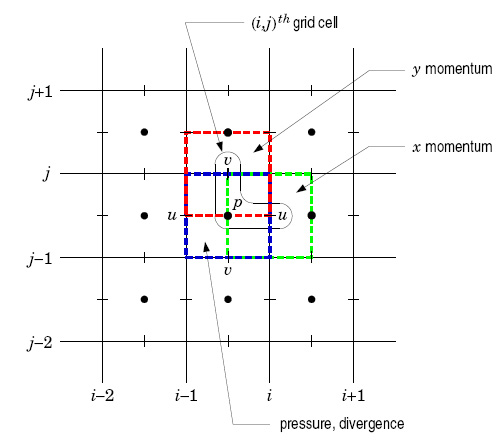
\includegraphics[width=9cm]{jiaocuo.png}
	\caption{交错网格}
	\label{fig:C2jiao}
\end{figure}


以守恒形式的方程为例
\begin{equation}
	\begin{aligned}
		u_{t}=-p_{x}+\nu \Delta u \\
		v_{t}=-p_{y}+\nu \Delta v
	\end{aligned}
\end{equation}
时间离散:隐式 Euler , 除了压力梯度项; 空间中心差分或有限体
\begin{equation}
	\begin{aligned}
		\frac{u_{i, j+\frac{1}{2}}^{n+1}-u_{i, j+\frac{1}{2}}^{n}}{\tau} = & -\frac{p_{i+\frac{1}{2}, j+\frac{1}{2}}^{n+1}-p_{i-\frac{1}{2}, j+\frac{1}{2}}^{n+1}}{h_{x}}+\nu \frac{u_{i+1, j+\frac{1}{2}}^{n+1}-2 u_{i, j+\frac{1}{2}}^{n+1}+u_{i-1, j+\frac{1}{2}}^{n+1}}{h_{x}^{2}} \\
		                                                                   & +\nu \frac{u_{i, j+\frac{3}{2}}^{n+1}-2 u_{i, j+\frac{1}{2}}^{n+1}+u_{i, j-\frac{1}{2}}^{n+1}}{h_{y}^{2}},
	\end{aligned}
	\label{eq:C2u}
\end{equation}
\begin{equation}
	\begin{aligned}
		\frac{v_{i+\frac{1}{2}, j}^{n+1}-v_{i+\frac{1}{2}, j}^{n+1}}{\tau} = & -\frac{p^{n+1}_{i+\frac{1}{2}, j+\frac{1}{2}}-p_{i+\frac{1}{2}, j-\frac{1}{2}}^{n+1}}{h_{y}}+\nu \frac{v_{i+\frac{3}{2}, j}^{n+1}-2 v_{i+\frac{1}{2}, j}^{n+1}+v_{i-\frac{1}{2}, j}^{n+1}}{h_{x}^{2}} \\
		                                                                     & +\nu \frac{v_{i+\frac{1}{2}, j+1}^{n+1}-2 v_{i+\frac{1}{2}, j}^{n+1}+v_{i+\frac{1}{2}, j-1}^{n+1}}{h_{y}^{2}}.
	\end{aligned}
	\label{eq:C2v}
\end{equation}
% 其中 $h_{x}$ 和 $h_{y}$ 是常数, 各种平均量定义为 $(x, y$ 方向的平均表示为 $\bar{*}, \widetilde{*})$
% \begin{equation}
% 	\begin{aligned}
% 		\bar{u}_{i+\frac{1}{2}, j+\frac{1}{2}}=\frac{1}{2}\left(u_{i+1, j+\frac{1}{2}}+u_{i, j+\frac{1}{2}}\right), \quad \widetilde{u}_{i, j}=\frac{1}{2}\left(u_{i, j+\frac{1}{2}}+u_{i, j-\frac{1}{2}}\right) \\
% 		\bar{v}_{i, j}=\frac{1}{2}\left(v_{i+\frac{1}{2}, j}+v_{i-\frac{1}{2}, j}\right), \quad \widetilde{v}_{i+\frac{1}{2}, j+\frac{1}{2}}=\frac{1}{2}\left(v_{i+\frac{1}{2}, j+1}+v_{i+\frac{1}{2}, j}\right)
% 	\end{aligned}
% \end{equation}
% 各个平均值都采用$n+1$时刻的点。

计算动量方程的散度:
\begin{equation}
	\Delta p=\nu \Delta D-D_{t}
\end{equation}
这里 $D \triangleq u_{x}+v_{y} .$ 和不保持速度散度自由性质那样, 不包含 $D_{t}$ 也会导致动 量方程解的非线性不稳定性. 项 $\nu \Delta D$ 似乎是可以略去, 特别是 当Reynolds数比较大时.
% (这里的做法不像在其它地方推导压力Poisson方 程那样先假设速度场是无散度的!)

在点 $i+\frac{1}{2}, j+\frac{1}{2}$ 处离散, 得
\begin{equation}
	\left(D_{0, x}^{2}+D_{0, y}^{2}\right) p^{n+1}=  \nu\left(D_{0, x}^{2}+D_{0, y}^{2}\right) D^{n}-\frac{D^{n+1}-D^{n}}{\tau},
\end{equation}
其中
\begin{equation}
	\begin{aligned}
		D_{0, x}^{2} p_{i+\frac{1}{2}, j+\frac{1}{2}} & =\frac{p_{i+\frac{3}{2}, j+\frac{1}{2}}-2 p_{i+\frac{1}{2}, j+\frac{1}{2}}+p_{i-\frac{1}{2}, j+\frac{1}{2}}}{h_{x}^{2}} \\
		D_{0, y}^{2} p_{i+\frac{1}{2}, j+\frac{1}{2}} & =\frac{p_{i+\frac{1}{2}, j+\frac{3}{2}}-2 p_{i+\frac{1}{2}, j+\frac{1}{2}}+p_{i+\frac{1}{2}, j-\frac{1}{2}}}{h_{y}^{2}}
	\end{aligned}
\end{equation}
因为希望在$t=t_{n+1}$时刻, 速度散度$D_{n+1} = 0$, 则离散的压力Poisson方程 变为
\begin{equation}
	\left(D_{0, x}^{2}+D_{0, y}^{2}\right) p^{n+1}=  \nu\left(D_{0, x}^{2}+D_{0, y}^{2}\right) D^{n}+\frac{D^{n}}{\tau},
\end{equation}
该方程中未知量仅为$p_{n+1}$. 结合适当的边界条件, 由该方程可解出$p_{n+1}$,



对于初始条件$\bm{u}(x, y, 0)=\bm{u}_{0}(x, y), \  (x, y) \in \Omega,$ 可以取交错网格上的点作为初始条件。而对于边界条件$\bm{u}(x, y, t)=\bm{u}_{b}(x, y), \  (x, y) \in \partial \Omega,\ t \geq 0$,可以取最靠近边界的$u,v$的值为给定点的边界条件。



接下来我们来看从数值格式得到涡流方程的数值格式的过程,根据涡的定义
\begin{equation}
	\omega = \partial_x v - \partial_y u
\end{equation}
用边上的速度点差分来得到网格上的涡量
\begin{equation}
	\omega_{ij} = \frac{v_{i+\frac{1}{2},j}-v_{i-\frac{1}{2},j}}{h_x} - \frac{u_{i,j+\frac{1}{2}}-u_{i,j-\frac{1}{2}}}{h_y}
\end{equation}
对\cref{eq:C2v,eq:C2u}分别沿着$x,y$方向移动一位置,然后相减再除以$h_x,h_y$,即作用$\Delta_x/h_x,\Delta_y$的算符后再相减可以构造出涡量的离散方程,注意压强在四点的取值在最后相减的一步正好抵消,所以最终离散的方程没有压强,
\begin{equation}
	\frac{\omega^{n+1}_{i,j}-\omega^{n}_{i,j}}{\tau}  =\nu  \frac{\omega_{i+1, j+\frac{1}{2}}^{n+1}-2 \omega_{i, j}^{n+1}+\omega_{i-1, j}^{n+1}}{h_{x}^{2}}+\nu \frac{\omega_{i, j+1}^{n+1}-2 \omega_{i, j}^{n+1}+\omega^{n+1}_{i, j-1}}{h_{y}^{2}},
\end{equation}
求出涡流后,再来求流函数
\begin{equation}
	\Delta_{h} \psi^{n+1} = -\omega^{n+1}
\end{equation}
其中$\Delta_{h}$ 是离散的五点 Laplace 算子,边界条件
\begin{equation}
	\left\{\begin{aligned}
		\left.\psi^{n+1}\right|_{\Gamma}       & =\psi_{b}  \\
		\left.D_{n} \psi^{n+1}\right|_{\Gamma} & =-v_{\tau}
	\end{aligned}\right.
\end{equation}


\subsection{3}

二维不可压缩流动的计算,可以通过引入流函数来使得速度散度为零的不可压缩条件自动满足,而涡量和流函数通过 Poisson 方程联系在一起,求解的方程组为如下的涡量流函数方程
\begin{equation}
	\left\{\begin{aligned}
		\frac{\partial \omega}{\partial t}          & =\nu \Delta \omega                 \\
		\Delta \psi                                 & =-\omega                           \\
		u=\frac{\partial \psi}{\partial y}, \quad v & =-\frac{\partial \psi}{\partial x}
	\end{aligned}\right.
	\label{eq:C31}
\end{equation}


边界条件一般是给出壁面的流函数值或者其法向导数值 (也就是切向速度)
\begin{equation}
	\psi=\psi_{b}, \quad \frac{\partial \psi}{\partial n}=-\bm{u}_{\tau}
\end{equation}
注意这里的切方向 $\tau$ 是流动区域的内法向量 ${n}$ 逆时针旋转 $90^{\circ}$ 的结果,这只是一种约定,也
可以规定法向量顺时针旋转 $90^{\circ}$ 得到切向量,那么公式中某些项的符号会有差异,在具体的
\begin{equation}
	\frac{\partial \psi}{\partial n}=-\bm{u}_{\tau}, \quad \frac{\partial \psi}{\partial \tau}=\bm{u}_{n}
\end{equation}
对于微分方程 \cref{eq:C31},空间导数项可以用通常的中心差分格式离散
\begin{equation}
	\left\{\begin{aligned}
		\frac{\dif \omega}{\dif t} & =\nu \Delta_{h} \omega \\
		\Delta_{h} \psi            & =-\omega
	\end{aligned}\right.
\end{equation}
其中 $D_{x}, D_{y}$ 是标准的中心差分格式, $\Delta_{h}$ 是离散的五点 Laplace 算子。 对时间导数采用向前 Euler 法 (在实际的计算中,只要有基本的向前 Euler 法,就可以
用 Runger-Kutta 等方法来通过多步计算来提高计算精度和格式的稳定性),此方程对内点的
离散格式为
\begin{equation}
	\left\{\begin{aligned}
		\frac{\omega^{n+1}-\omega^{n}}{\tau}   & =\nu \Delta_{h} \omega^{n} \\
		\Delta_{h} \psi^{n+1}                  & =-\omega^{n+1}             \\
		\left.\psi^{n+1}\right|_{\Gamma}       & =\psi_{b}                  \\
		\left.D_{n} \psi^{n+1}\right|_{\Gamma} & =-v_{\tau}
	\end{aligned}\right.
\end{equation}
或者也可以采用隐式格式。先求涡量,再求流函数,可以发现离散后和的格式和上一问得出的离散格式是一样的。




\nocite{*}

\bibliographystyle{plain}

\phantomsection

\addcontentsline{toc}{section}{参考文献} %向目录中添加条目,以章的名义
\bibliography{homework}

\end{document}

